The clustering approach was used to minimize the constraints imposed by scattered and distant population and cropland points. Forty clusters were created (\Fref{fig:clusters}) in the process, which succeeded in identifying dense agglomerations. When compared with a traditional approach of performing an analysis on a province basis, the clusters achieved a reduction of 347\% on the overall distance between points.

\begin{figure*}[!h]
    \centering
	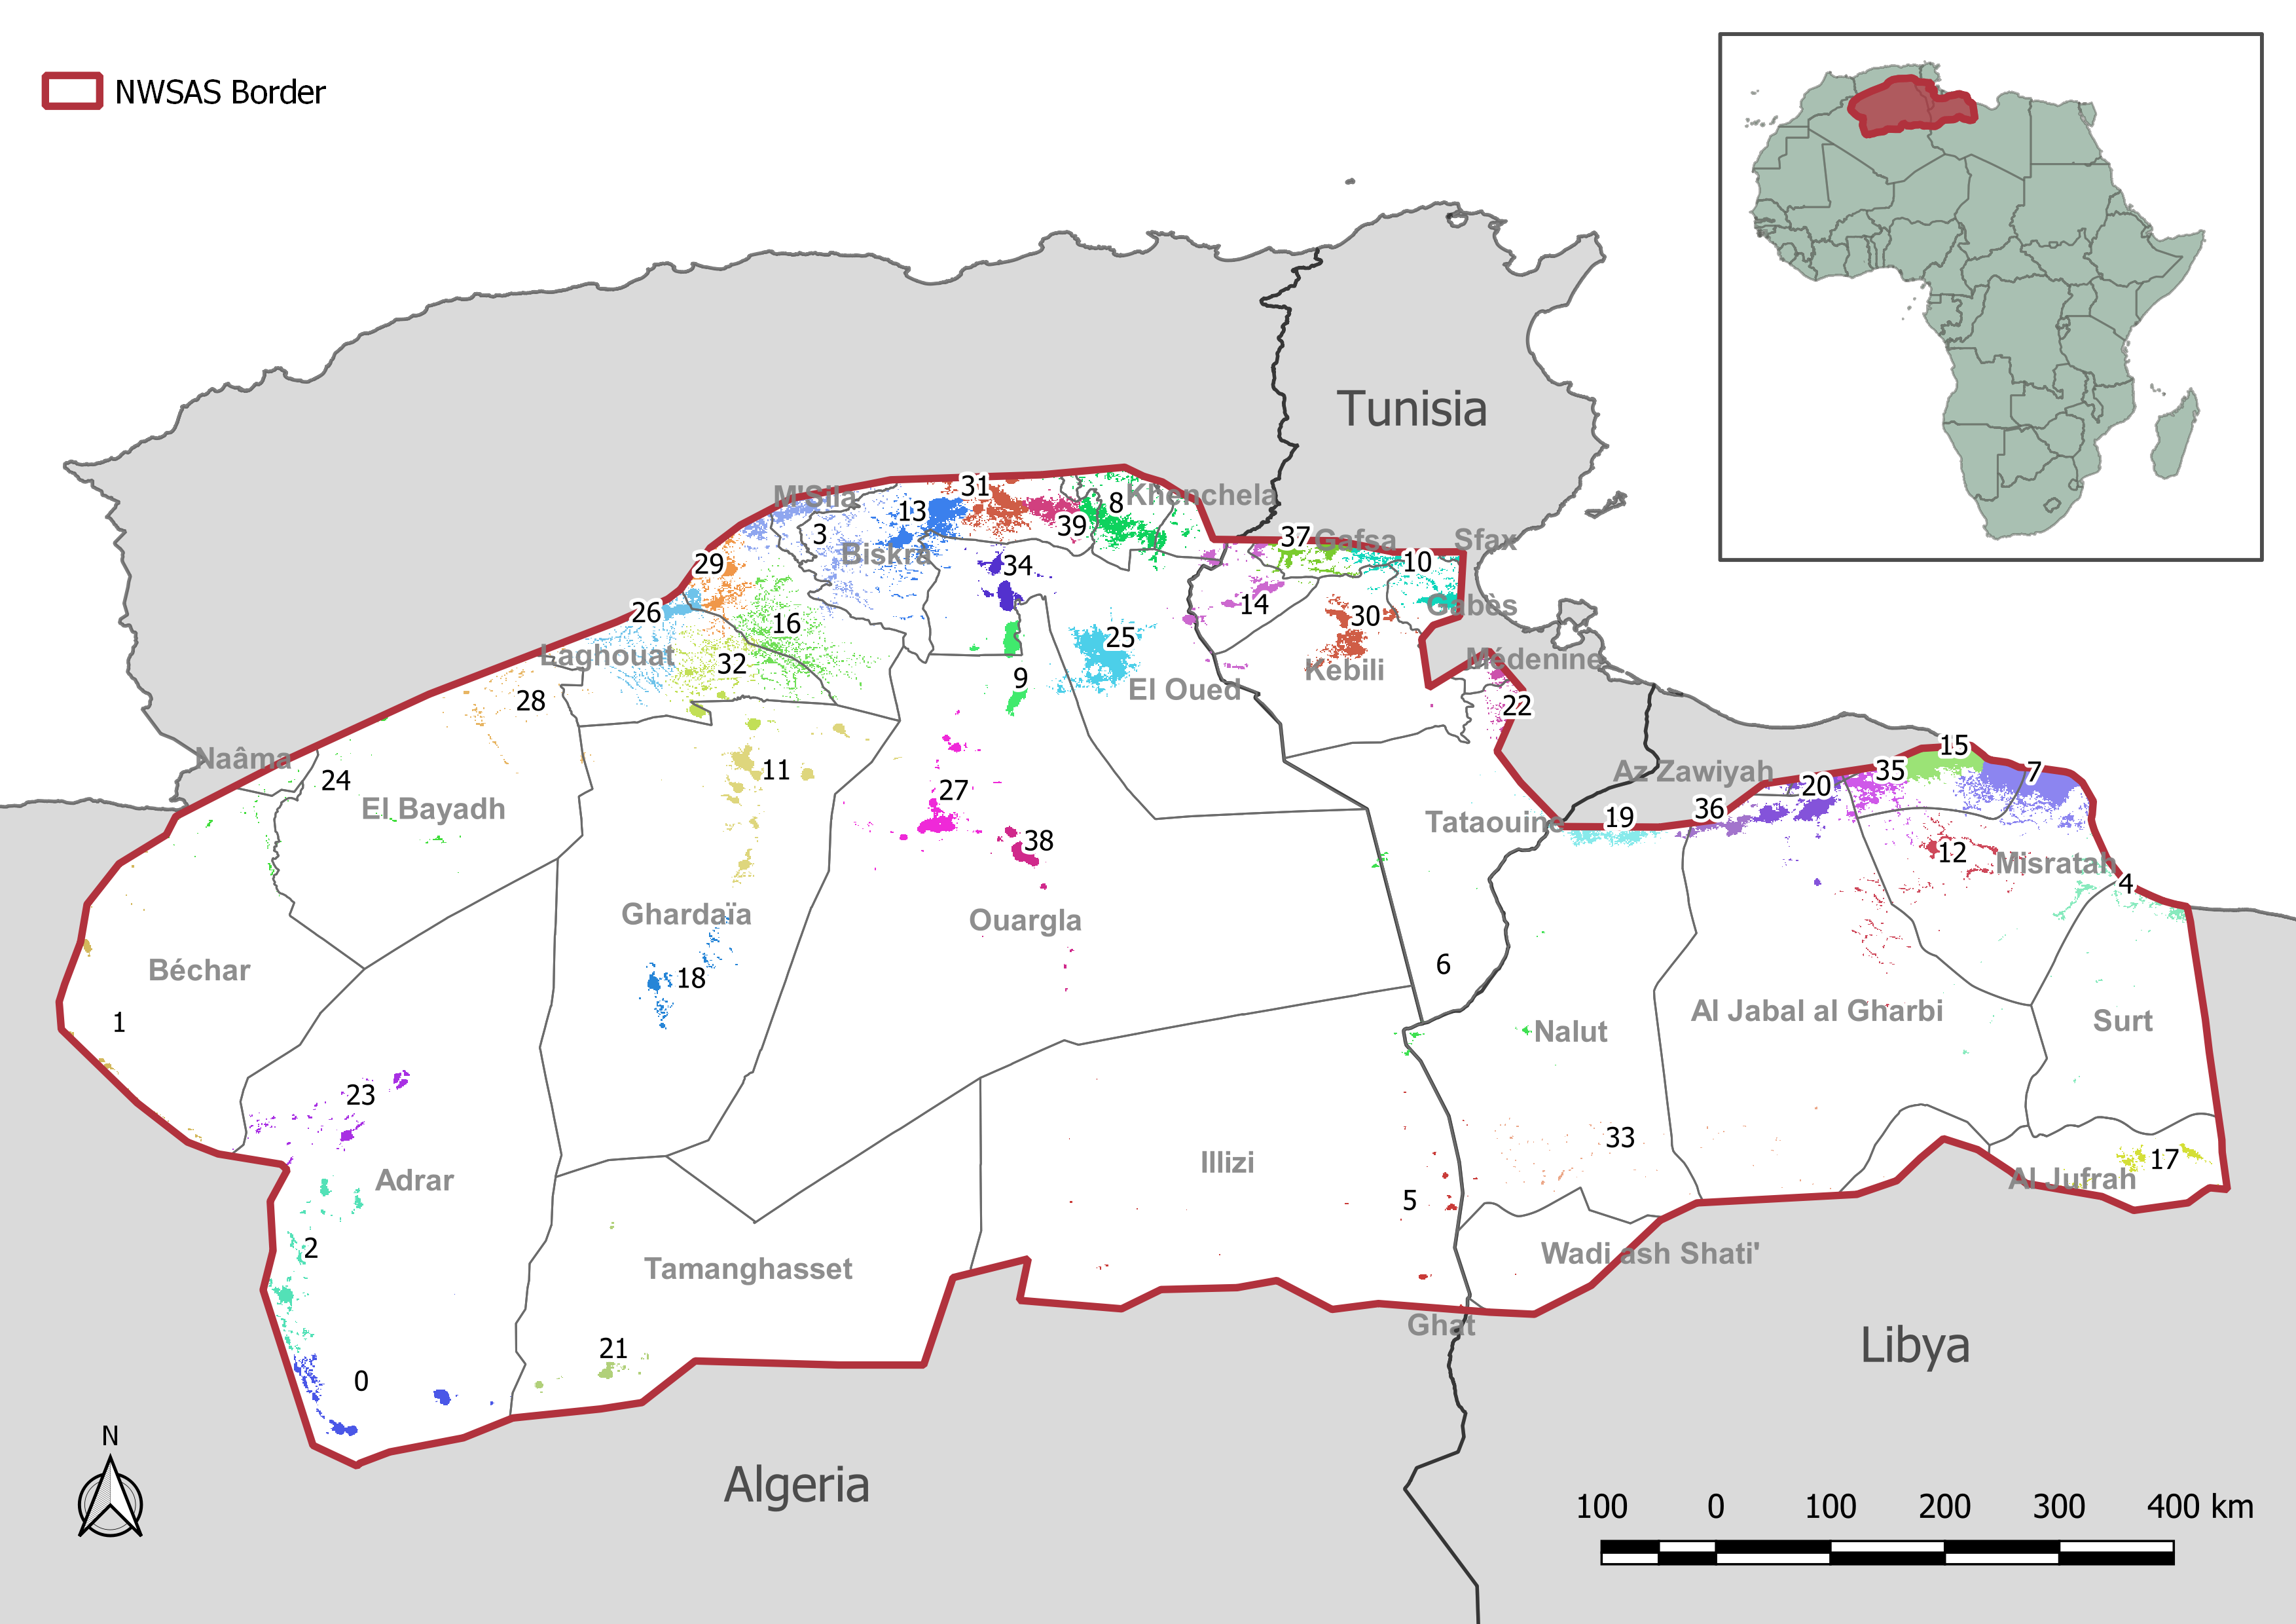
\includegraphics[width=0.88\textwidth, cfbox=black 1pt 0pt]{NWSAS_clusters}
	\caption{Population and cropland clusters. Clusters are numbered from 0 to 39, yielding 40 agglomerations including each population and cropland areas. Every cluster is tagged with a number and colored to make them stand out from others. The grey administrative boundaries correspond to the different provinces.}
	\label{fig:clusters}
\end{figure*}

This is especially important in larger provinces with substantial population and agricultural activity as Adrar, Ghardaïa, Ouargla el Oued and Misratah. Moreover, with this approach, the administrative border constraint is eliminated, as can be seen with cluster number 9 where the agglomeration shares areas from the Ouargla and El Oued provinces. 
% This implies an interesting question for the need of collaboration between provinces and even countries.

Water use in the Baseline scenario was estimated at 5,913 Mm\textsuperscript{3}/yr, agricultural irrigation accounting for 94\% share (see \fref{fig:water}). In the water reuse scenario with private agricultural water regime, the overall water use was lower than the baseline, opposite behaviour to the subsidized and free agricultural water schemes. However, due to the reused water share in the subsidized regime, the overall water extractions were lower than those of the Baseline and close to the ones from the private regime. This suggests that either with the use of more efficient irrigation schemes (i.e. the private regime) or the use of lower efficiency irrigation coupled with water reuse (i.e. subsidized regime), similar results could be achieved.

\begin{figure*}[!ht]
	\centering
	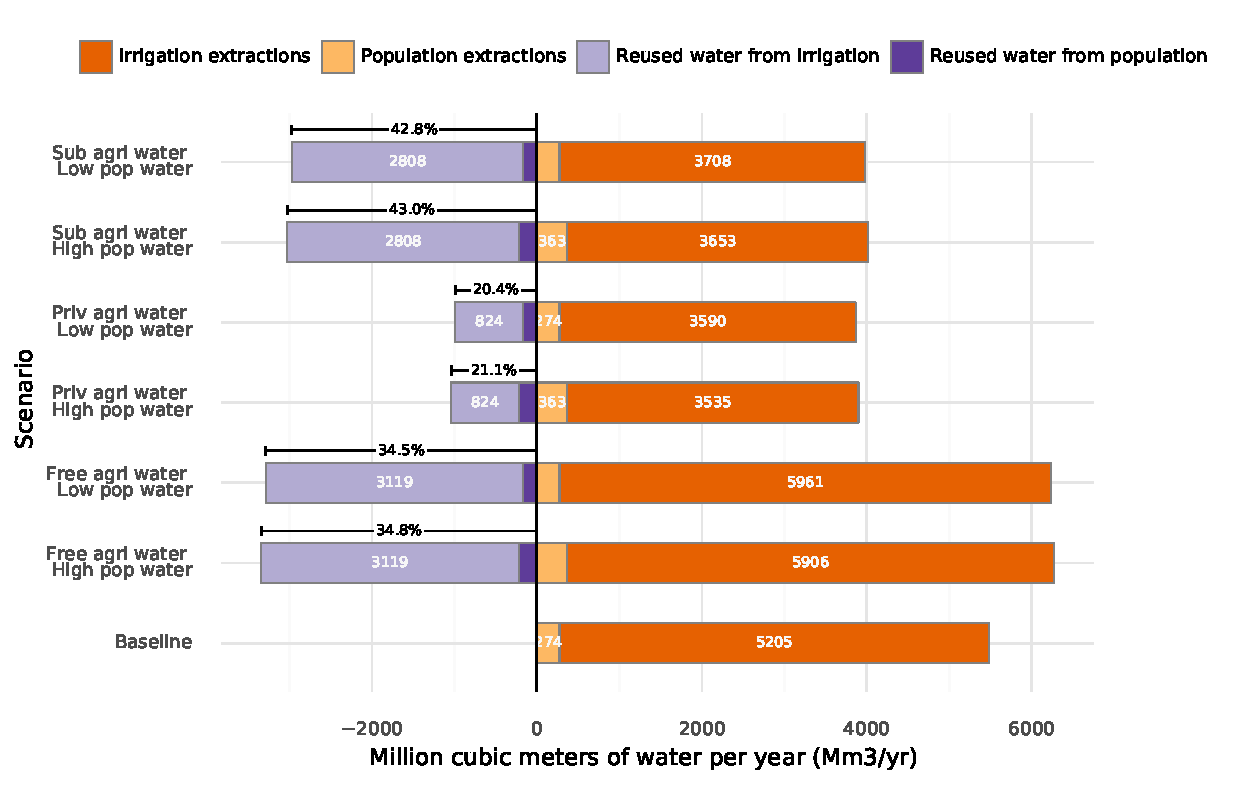
\includegraphics[width=\textwidth]{Water}
	\caption{Water usage for all scenarios. At left: reused water after reclaim, treatment and allocation classified by population and irrigation source. At right: overall water extractions classified by population and irrigation use. Percentage bars indicate the share of reused water against the total demand.}
	\label{fig:water}
\end{figure*}

On the other hand, the free agricultural water regime yielded much larger water extractions, even with water reuse. In fact, the share of reused water accounted for around 34\% of the water usage, lower share than that of the subsidized regime. This was due to the cap set to the on-farm storage area of maximum 2\% share of the cropland area. Therefore, while more recoverable water is available in the free water regime, the storage system cannot hold everything. This could be solved by setting a higher value for the permissible on-farm storage area, however, this would mean that more agricultural area would be lost for storage purposes which can affect the farmers' revenues.

Population water levels do not cause meaningful variations in the overall water use, as agricultural water needs are much more extensive. Nonetheless, with the use of more efficient irrigation schemes, the recoverable water from irrigation drainage decreases, thus populations treated wastewater share on agricultural water usage increases.

The Groundwater Stress Indicator was computed aggregating the entire aquifer area (\fref{fig:gws}). A value of 5.36 in the Baseline scenario was obtained, which falls inside the medium to high stress category---however, it is known that the stress level in some parts of this area can reach to the extremely high category \cite{herbertGlobalAssessmentCurrent2019}. The private and subsidized agricultural water scenarios, presented a Groundwater Stress Indicator in the category of low to medium stress, which suggests a success by the treated wastewater measure in reducing the stress on the resource. However, the outcomes obtained for the free agricultural water scenarios, are higher at 5.72 and 5.77. Such increase in the stress, is due to the higher water requirements for agricultural irrigation.

\begin{figure}[!h]
	\centering
	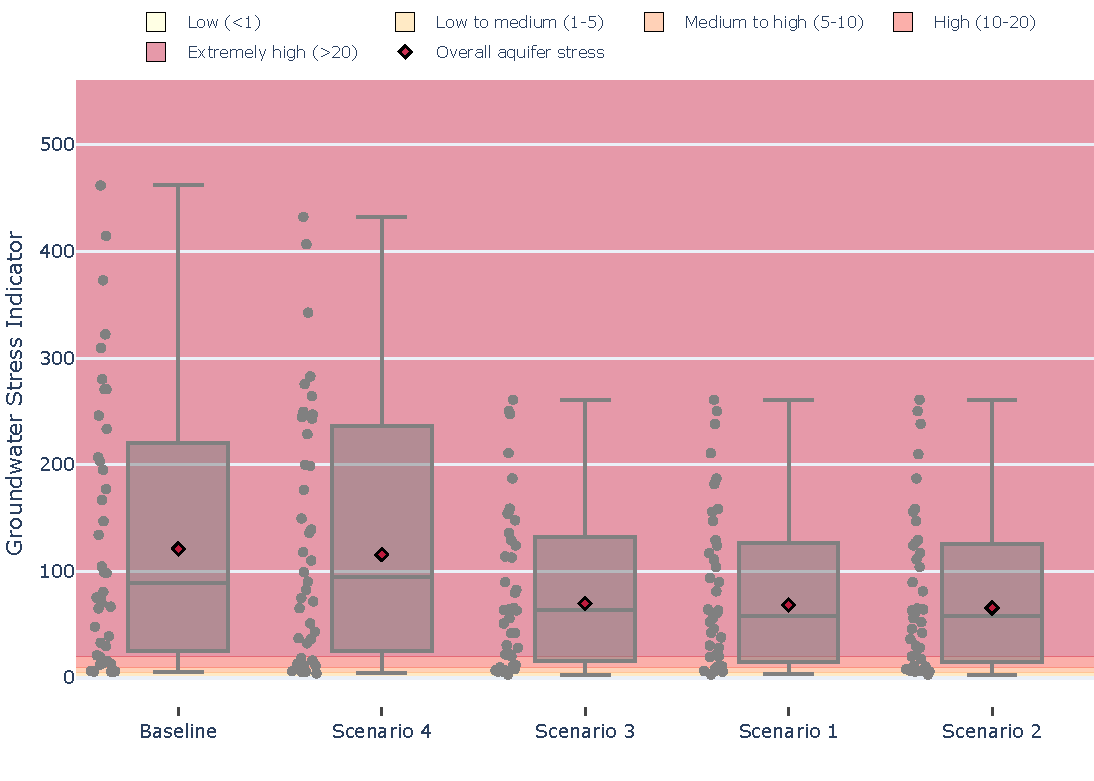
\includegraphics[width=0.7\textwidth]{GWS}
	\caption{Groundwater stress indicator for all scenarios.}
	\label{fig:gws}
\end{figure}

The least-cost treatment systems obtained for the low and high population water scenarios, share similarities in the combination of technologies identified (\fref{fig:leastLow} and \fref{fig:leastHigh}). Extended aeration, rotating biological contractors and intermittent sand filter were the least-costly technologies chosen. Nonetheless, differences in the technology shares exist. In the low population water requirements scenarios, wastewater was treated by intermittent sand filters, rotating biological contractors and extended aeration by 4\%, 21\% and 75\% share respectively. Whereas, in the high population water requirements scenario this shares were 2\%, 11\% and 87\%. In general, when lower capacity is required simpler treatment technologies are more cost-effective, as the independent variable of the CAPEX and OPEX cost functions is the available reclaimed wastewater flow.

\begin{figure*}[!ht]
	\centering
	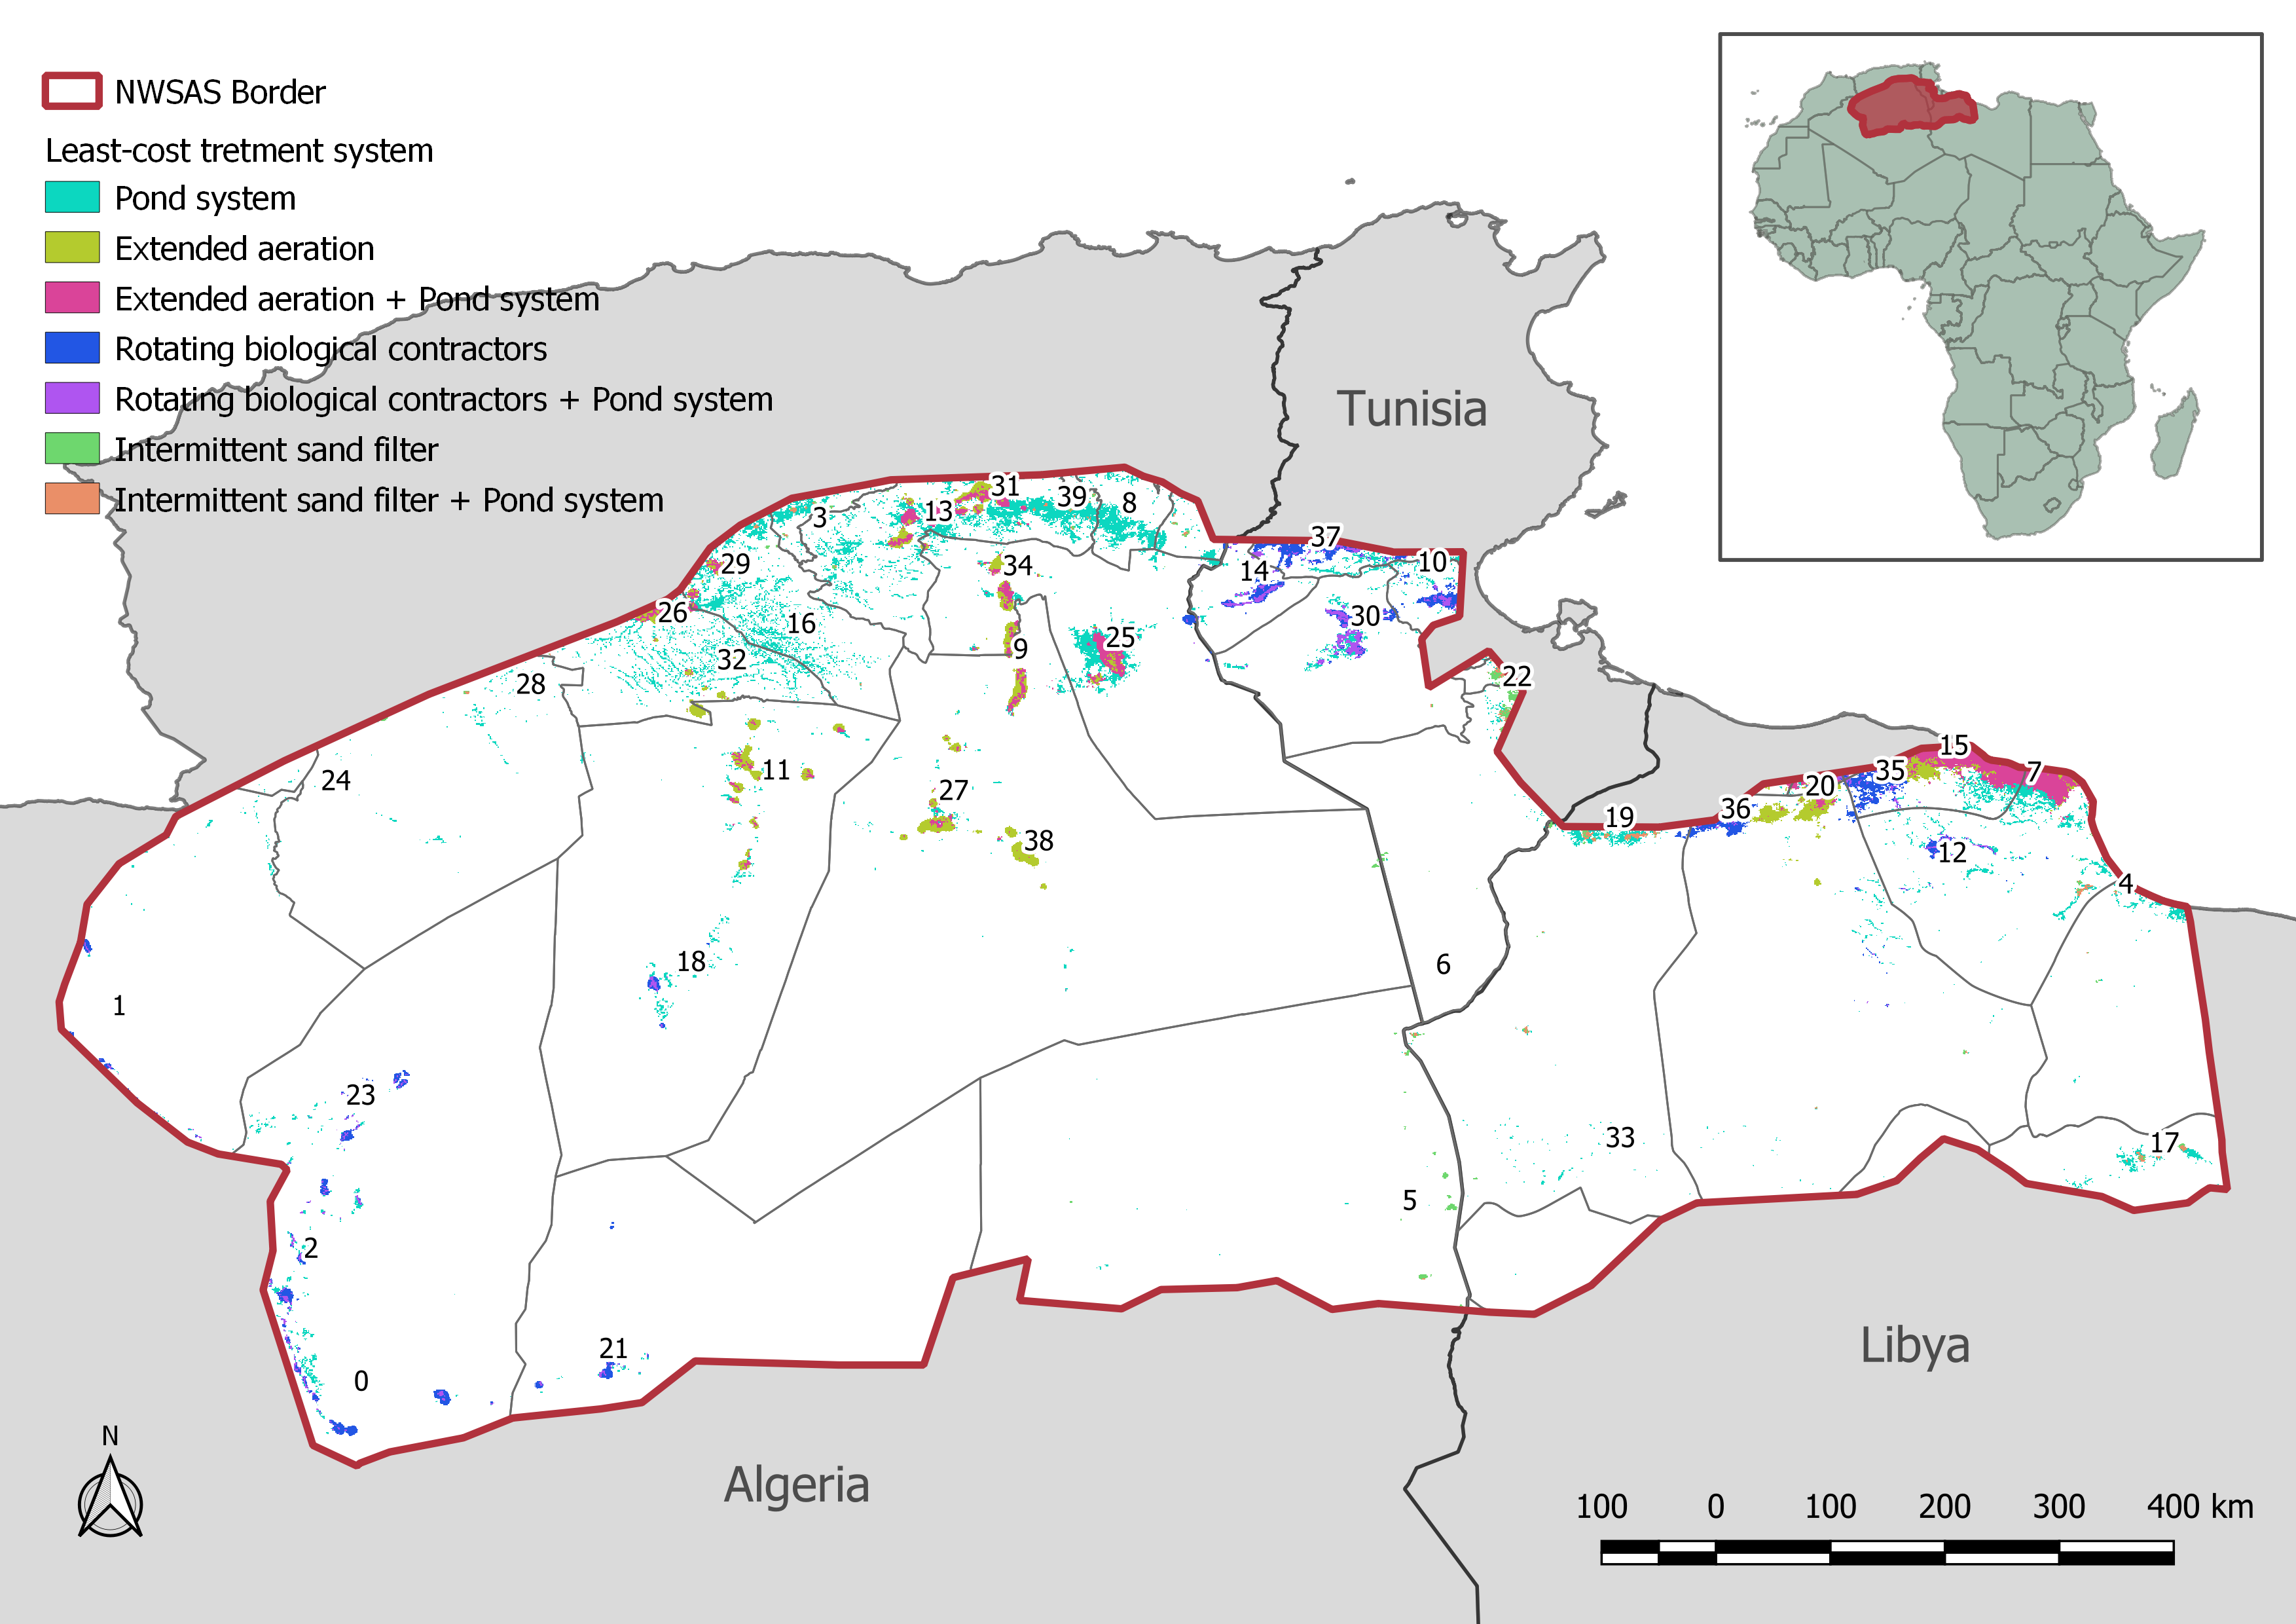
\includegraphics[width=0.88\textwidth, cfbox=black 1pt 0pt]{NWSAS_least-cost_system_cluster}
	\caption{Least-cost wastewater treatment options per cluster---low population water requirements.}
	\label{fig:leastLow}
\end{figure*}

\begin{figure*}[!ht]
	\centering
	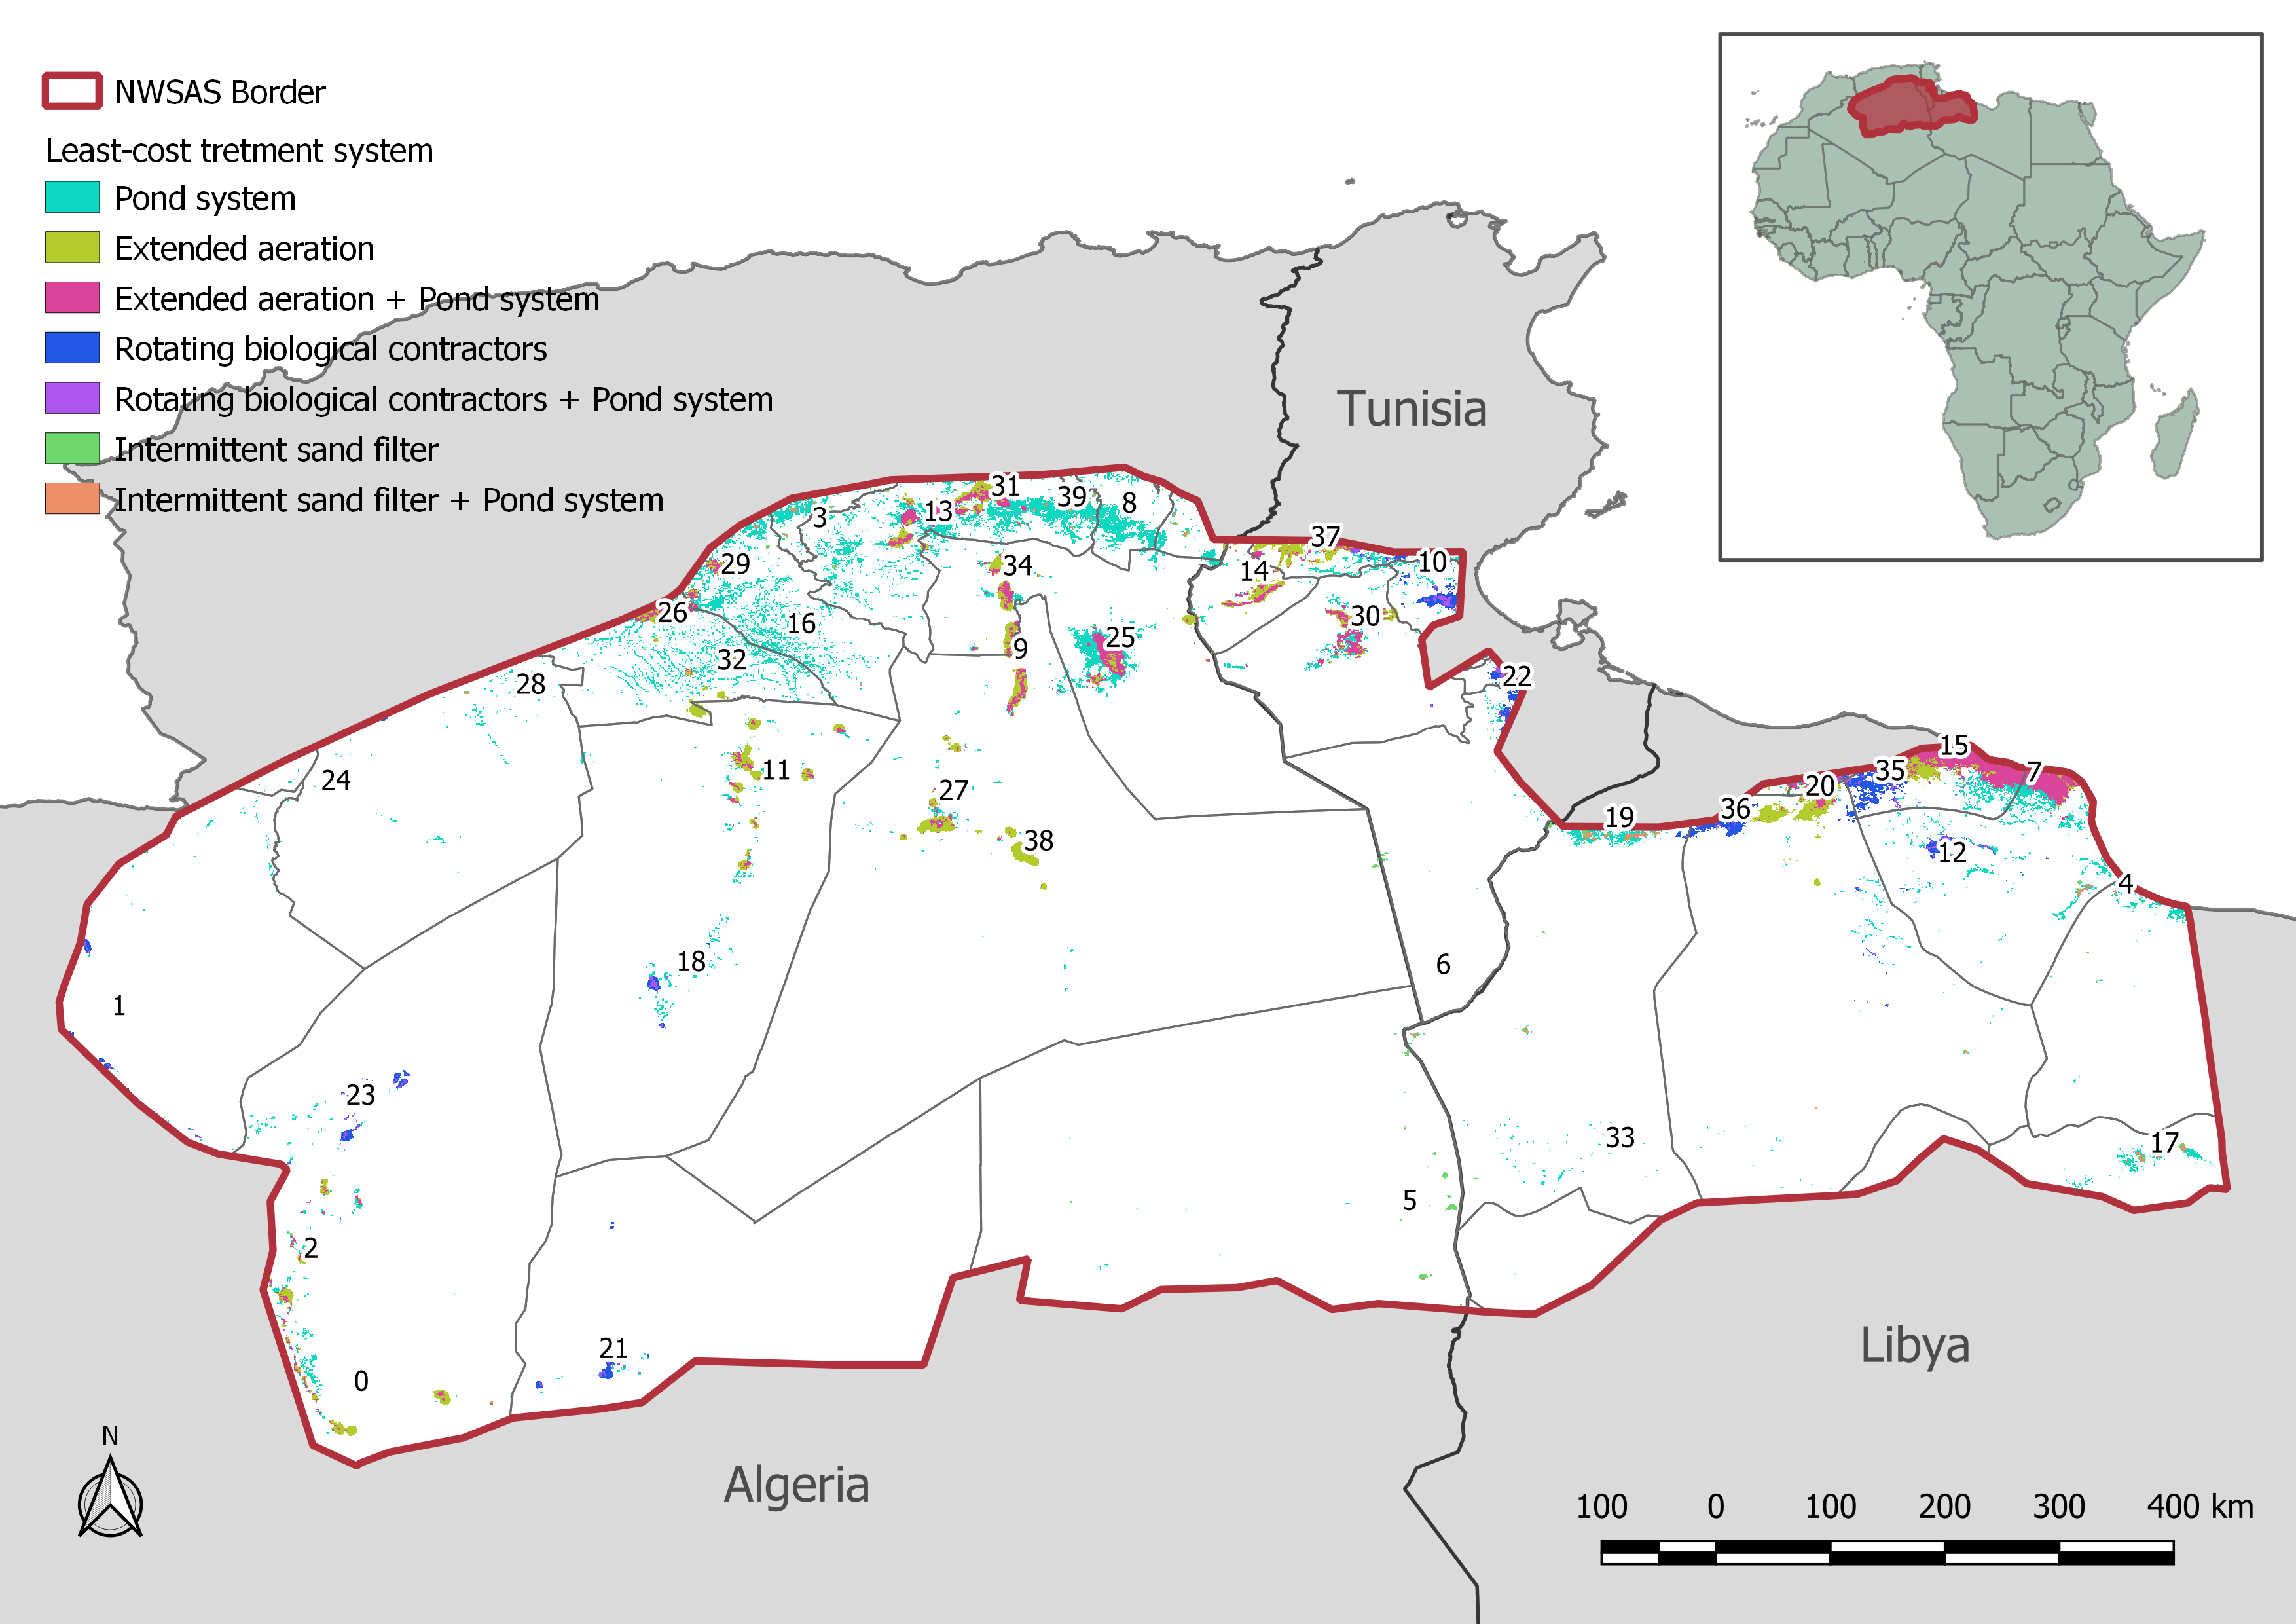
\includegraphics[width=0.88\textwidth, cfbox=black 1pt 0pt]{NWSAS_least-cost_system_cluster_high}
	\caption{Least-cost wastewater treatment options per cluster---high population water requirements.}
	\label{fig:leastHigh}
\end{figure*}

The previous is important, as the amount of wastewater available from the agglomerations is key for the calculation of the least costly technology. Therefore, with larger agglomerations, scalable and higher capacity systems could be implemented. The downside however, is that if the costs related to the conveyance system are not evaluated, then the distances among population and/or irrigation points become irrelevant, which is arguably far from reality. Thus, the analysis of more compact clusters, reduces the drawbacks of not calculating the costs related to a wastewater conveyance system.

Overall, the least-cost treatment systems obtained, show an important trade-off, as the best solution is dependent from geospatial factors than can render a specific technology less costly than other in a given region. For example, clusters 0, 2, 37, 30 and 14 use rotating biological contractors in the low population water requirements scenarios, whereas extended aeration in the high population water scenario. Similarly, cluster 22 passes from using intermittent sand filters to biological rotating contractors.

\begin{figure*}[!b]
	\centering
	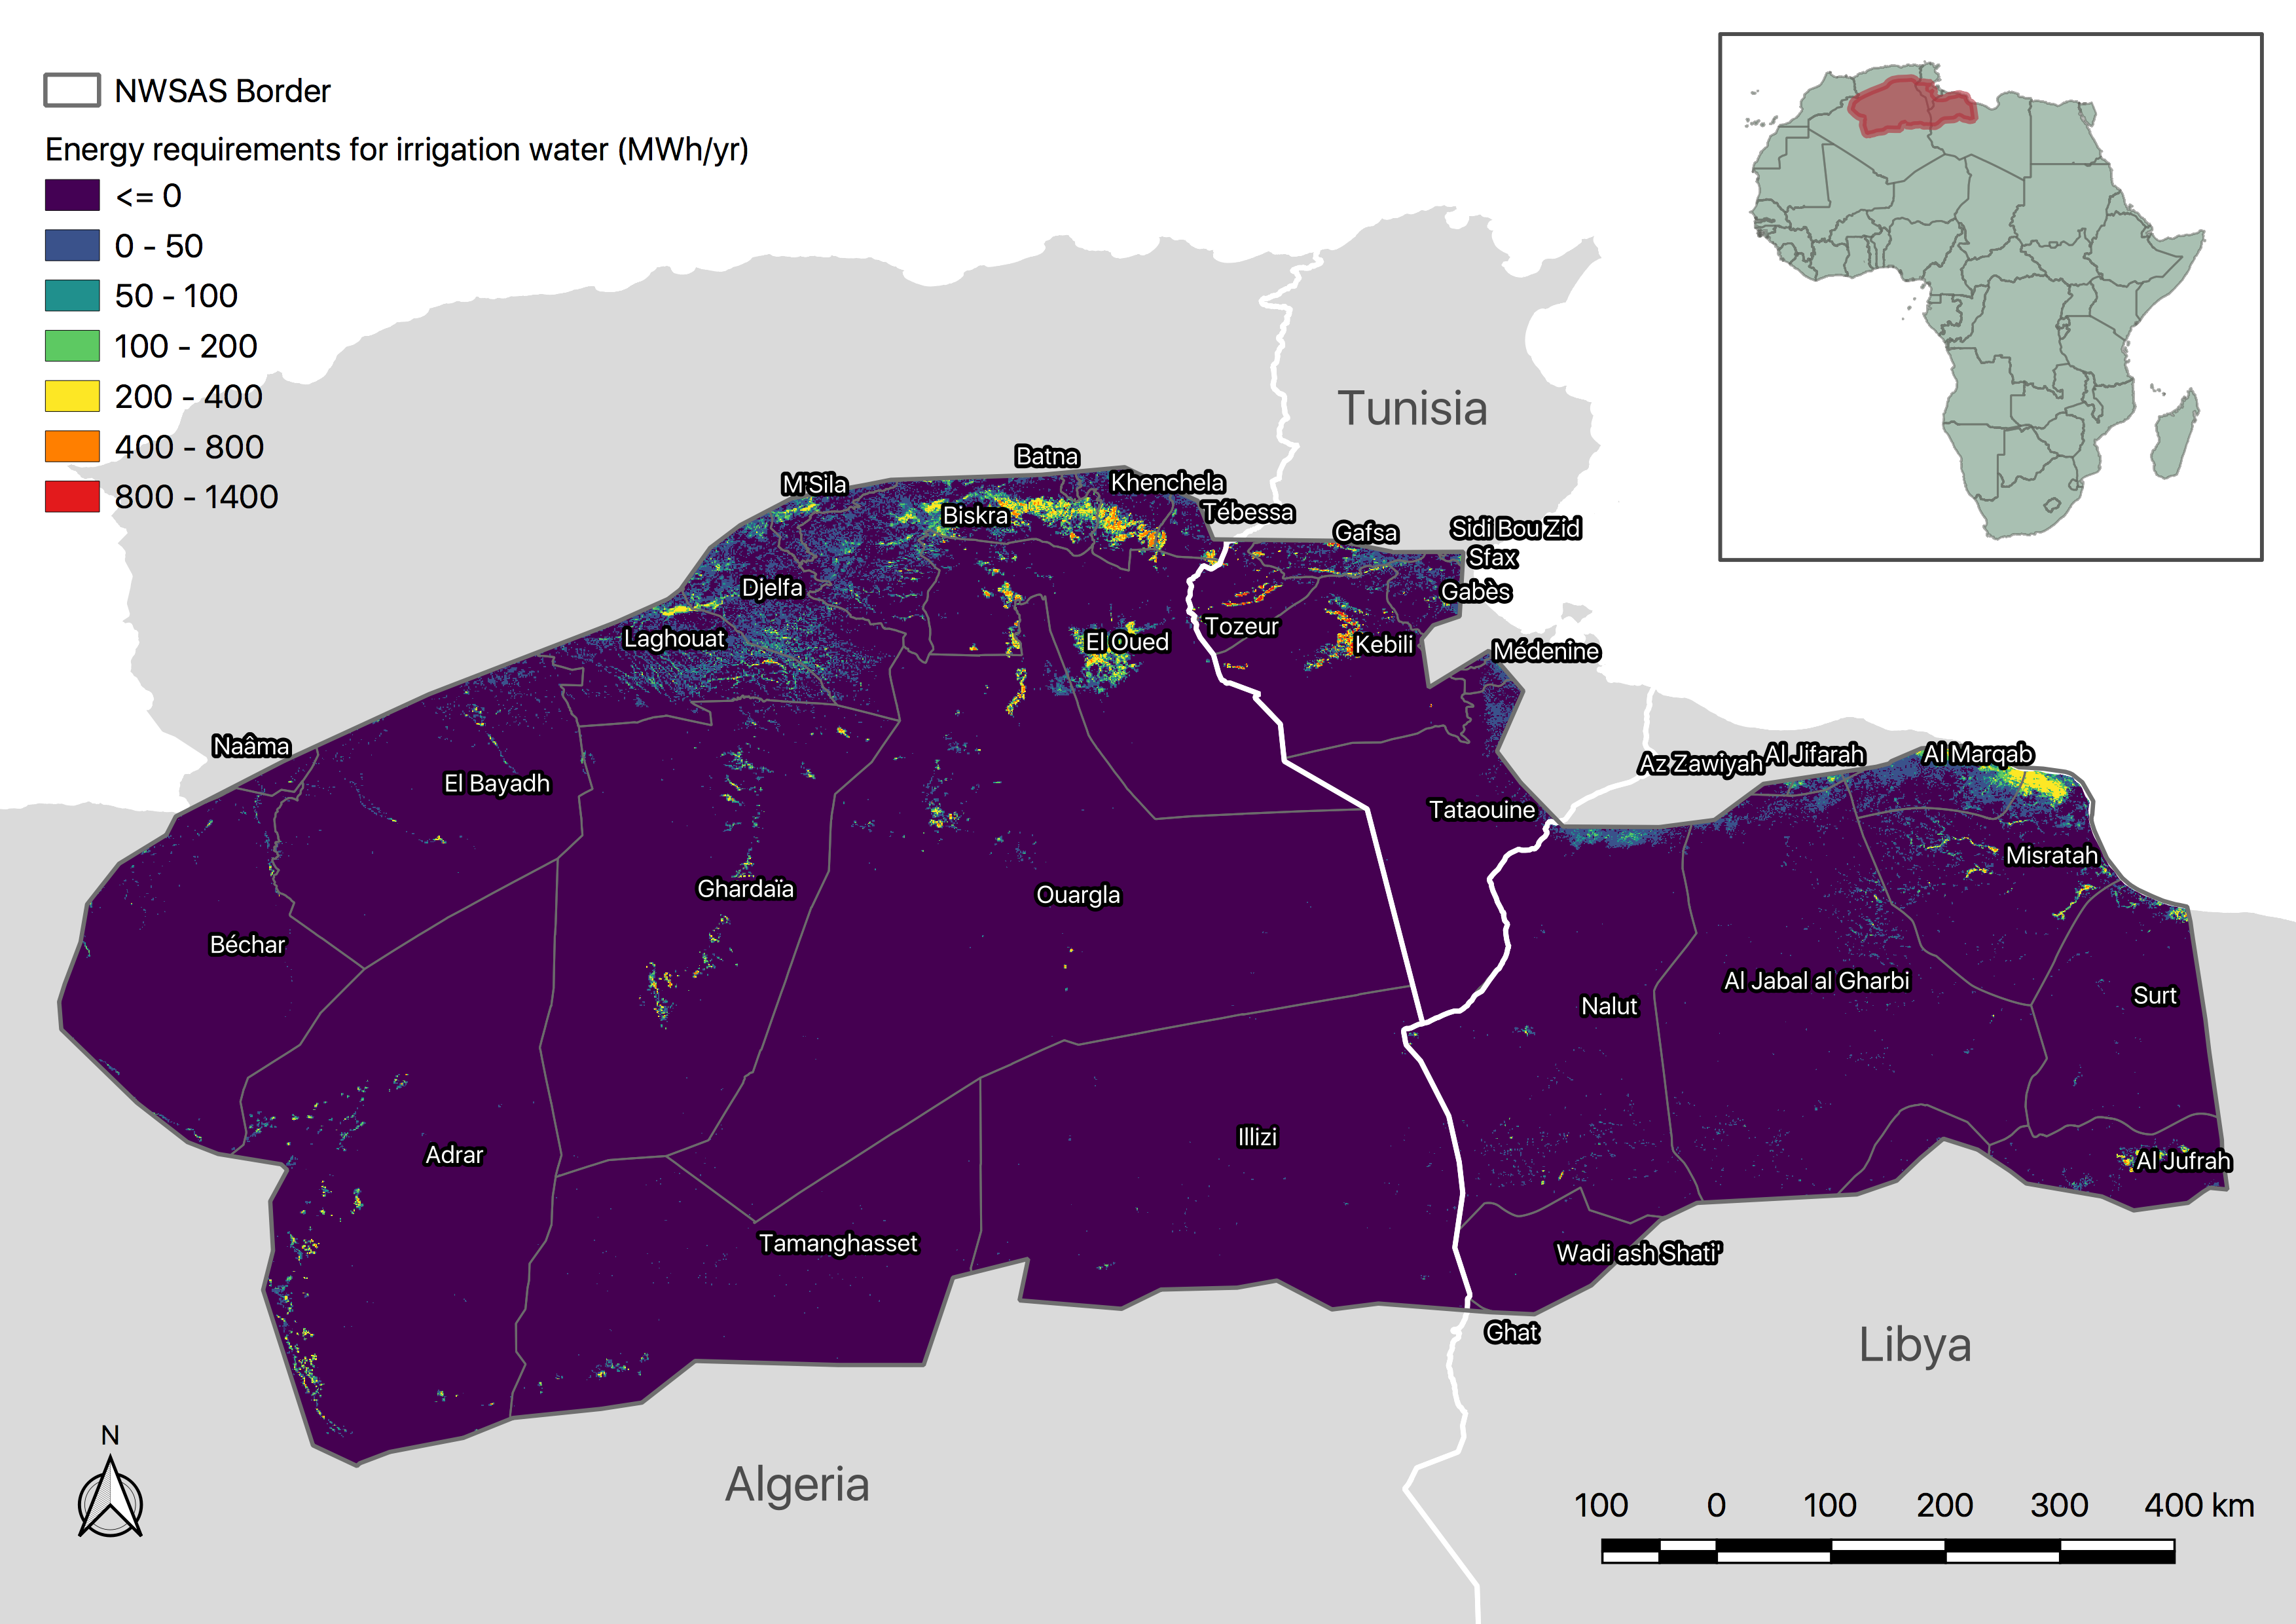
\includegraphics[width=0.88\textwidth, cfbox=black 1pt 0pt]{NWSAS_Energy_map}
	\caption[NWSAS energy used for irrigation water map - Baseline scenario]{North Western Sahara Aquifer System - Energy used for irrigation water map - Baseline scenario.}
	\label{fig:energy_map}
\end{figure*}

Yearly pumping energy requirements for agricultural water are shown in \fref{fig:energy_map}. The energy demand is considerably larger for Algeria and Tunisia in the northern parts of the aquifer. This is due to the higher average water demand per hectare existent in Algerian and Tunisian (according to statistics), the higher salinity contents found in this areas and the intense agricultural activity. On the other hand, the Al Marqab and Misratah provinces in Libya, present medium range energy consumption, even though the agricultural activity there is considerably high. Moreover, the energy needs for agricultural irrigation in the Adrar province, are in the medium to high range, although cropland density is much lower compared to the northern provinces. This suggests that, the deeper water table levels found along the province, can significantly affect the pumping energy requirements, impacting as well the water productivity of the region.

The overall energy related outcomes for all scenarios are shown in \fref{fig:energy}. The energy requirements for groundwater pumping represent the major part of all three activities. Desalination energy, although considerable, is much smaller than pumping energy, this mainly due to the medium TDS levels found throughout the groundwater aquifer. All scenarios apart from the free agricultural water ones, reduced overall energy consumption compared to the Baseline. Such reductions, are achieved by the reuse of treated wastewater in irrigation, as the energy intensity of treatment is substantially lower than the energy intensity for pumping water from the deep aquifer.

\begin{figure*}[!t]
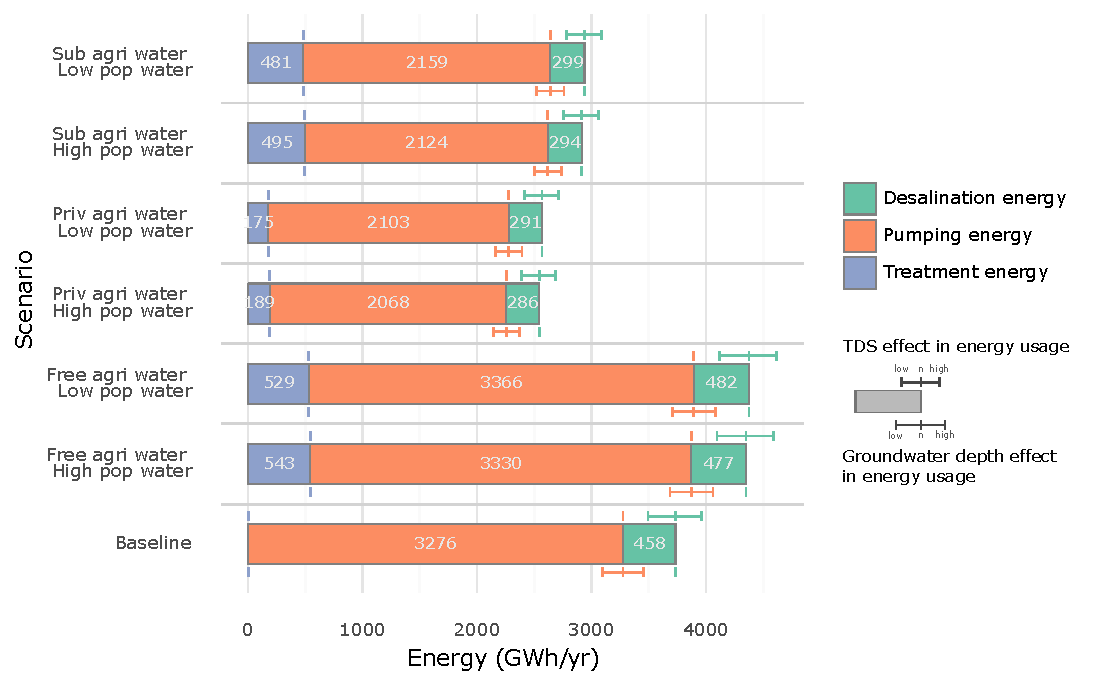
\includegraphics[width=\textwidth]{Energy}
\caption{Energy requirements for all scenarios with TDS and groundwater depth sensitivity analysis. TDS levels correspond to: $low=0.5\times n$ and $high=1.5\times n$; and groundwater depth levels correspond to: $low=n-10$ and $high=n+10$ meters.}
\label{fig:energy}
\end{figure*}

The sensitivity analysis demonstrates how a change of \rpm10 meters in the depth to groundwater level, has an average variation of circa \rpm5.5\% over the overall pumping energy requirements. Moreover, desalination energy requirements showed variations of $-$53\% to $+$50\%, when changes of \rpm50\% in the TDS levels were considered.

These effects on the energy-for-water requirements, are necessary to be assessed when planning for new water policies and water management strategies. Accordingly, accounting for new energy infrastructure, or potential energy savings could be key for the success of a new policy or solution to the water scarcity problem.